\documentclass{beamer}
\usepackage{caption}
\usepackage{etex}
\usepackage{amsmath,amsthm,fancyhdr,setspace,graphicx,booktabs,pdflscape}
\usepackage{geometry}
\usepackage{xcolor,colortbl}
\usepackage{url}
\usepackage{enumerate}
\usepackage{graphicx}
\usepackage{multicol}
\usepackage{caption}
\usepackage{tabularx}

\usepackage{beamerprosper}
\usepackage{pgfpages, pdfpages}
\usepackage{tikz-cd}
\usepackage{listings,fancyvrb}
\usepackage{hyperref}

\usetikzlibrary{er,positioning,calc,decorations.pathreplacing}

\mode<presentation>
\usefonttheme{structuresmallcapsserif}
\setbeamertemplate{footline}[frame number]{}
\setbeamertemplate{navigation symbols}{}

\newcommand{\fig}[3]{\begin{frame}\frametitle{#2}\centerline{\includegraphics[width=#3in]{#1}}\end{frame}}

\newcommand{\blackslide}[1]{\beamersetaveragebackground{black}\begin{frame}\frametitle{}\end{frame}\beamersetaveragebackground{white}}

\newcommand{\m}[2]{\begin{frame}\frametitle{#1}{ #2}\end{frame}}
\newcommand{\mm}[3]{\begin{frame}\frametitle{#1}\uncover<1->{ #2}\uncover<2->{ #3 }\end{frame}}
\newcommand{\mmm}[4]{\begin{frame}\frametitle{#1}\uncover<1->{ #2}\uncover<2->{ #3 }\uncover<3->{ #4 }\end{frame}}
\newcommand{\mmmm}[5]{\begin{frame}\frametitle{#1}\uncover<1->{ #2}\uncover<2->{ #3 }\uncover<3->{ #4 }\uncover<4->{ #5 }\end{frame}}

\setlength{\footskip}{24pt}

\newcommand{\ex}{\mathbf{E}}
\newcommand{\cov}{\mathbb{C}}
\newcommand{\var}{\mathbb{V}}
\newcommand{\tu}{\overline{\theta}}
\newcommand{\vu}{\overline{v}}
\newcommand{\tl}{\underline{\theta}}
\newcommand{\ab}{\bar{a}}
\newcommand{\lb}{\bar{L}}
\newcommand{\hb}{\bar{H}}
\newcommand{\btVFill}{\vskip0pt plus 1filll}

\newtheorem{proposition}{Proposition}
%\newtheorem{theorem}{Theorem}

\newenvironment{changemargin}[2]{%
    \begin{list}{}{ %
            \setlength{\topsep}{0pt}%
            \setlength{\leftmargin}{#1}%
            \setlength{\rightmargin}{#2}%
            \setlength{\listparindent}{\parindent}%
        \setlength{\itemindent}{\parindent}%
            \setlength{\parsep}{\parskip}%
        }%
\item[]}{\end{list}}

\newcommand<>{\g}[1]{{\color#2{gray} #1}}

% New colors.
\definecolor{darkred}{rgb}{0.6,0,0}
\definecolor{darkblue}{rgb}{.15,.25,.55}
\definecolor{darkgreen}{rgb}{0,.35,.05}
\definecolor{ltgreen}{rgb}{0,.05,.8}
\definecolor{bred}{rgb}{1,0,.05}
\definecolor{navy}{rgb}{.1,.1,.5}

% from beamer lecture 
\newcommand{\alrt}[1]{{\color{alert} #1}}
\newcommand{\alrtl}[1]{{\color{alert}\large #1}}
\newcommand{\alrtL}[1]{{\color{alert}\Large #1}}
\newcommand{\struc}[1]{{\color{structure} #1}}
\newcommand{\strucL}[1]{{\color{structure}\Large #1}}
\newcommand{\strucl}[1]{{\color{structure}\large #1}}
\newcommand{\dred}[1]{{\color{darkred} #1}}
\newcommand{\dredl}[1]{{\color{darkred}\large #1}}
\newcommand{\dredL}[1]{{\color{darkred}\Large #1}}
\newcommand{\altc}[1]{{\color{darkgreen}\textbf{#1}}}
\newcommand{\altcl}[1]{{\color{darkgreen}\textbf{\large #1}}}
\newcommand{\altcL}[1]{{\color{darkgreen}\textbf{\Large #1}}}
\newcommand{\hush}{\hushit}
\newcommand{\hushalrt}[1]{\hushit{{\color{alert} #1}}}
\newcommand{\hushalrtl}[1]{\hushit{{\large\color{alert} #1}}}
\newcommand{\hushalrtL}[1]{\hushit{{\Large\color{alert} #1}}}
\newcommand{\hushstruc}[1]{\hushit{{\color{structure} #1}}}
\newcommand{\hushstrucl}[1]{\hushit{{\large\color{structure} #1}}}
\newcommand{\hushstrucL}[1]{\hushit{{\Large\color{structure} #1}}}


\definecolor{themecolor}{RGB}{160, 82, 45}
\definecolor{darkgreen}{RGB}{160, 82, 45}
\definecolor{myblue}{RGB}{0, 139, 188}

\def \mainroot{..}
\def \figroot{\mainroot/figures/heatmaps}

\setbeamercolor{description item}{fg=themecolor!80!black}
\setbeamercolor{button}{fg=themecolor,bg=white}
\setbeamercolor{frametitle}{fg=themecolor}
\setbeamercolor{title}{fg=themecolor}
\setbeamercolor{caption name}{fg=themecolor}
\setbeamercolor{subtitle}{fg=themecolor}
\setbeamercolor{item}{fg=themecolor}
\setbeamercolor{itemize/enumerate body}{fg=black}  


\title{Heatmaps for Economic Analysis}
\author{Tom Cui, Eric Zwick \\ (DRAFT)}


\begin{document}

\begin{frame}
\titlepage
\end{frame}


\begin{frame}{What is a heatmap?}
        \begin{itemize}
                \item \altcl{A two-dimensional visualization of data using colour to represent magnitude}
             \item Broad definition, which could be divided into
             \item \textbf{Embedded} heatmaps that overlay colour on an actual map or image (not covered here)
             \item \textbf{Matrix} heatmaps that presents a grid of values where colours differ by cell
        \end{itemize}
\end{frame}

\begin{frame}{What is a heatmap?}
        \textbf{Example:} The WSJ vaccine visualization (DeBold, Friedman 2015)
    \begin{tikzpicture}
        \node {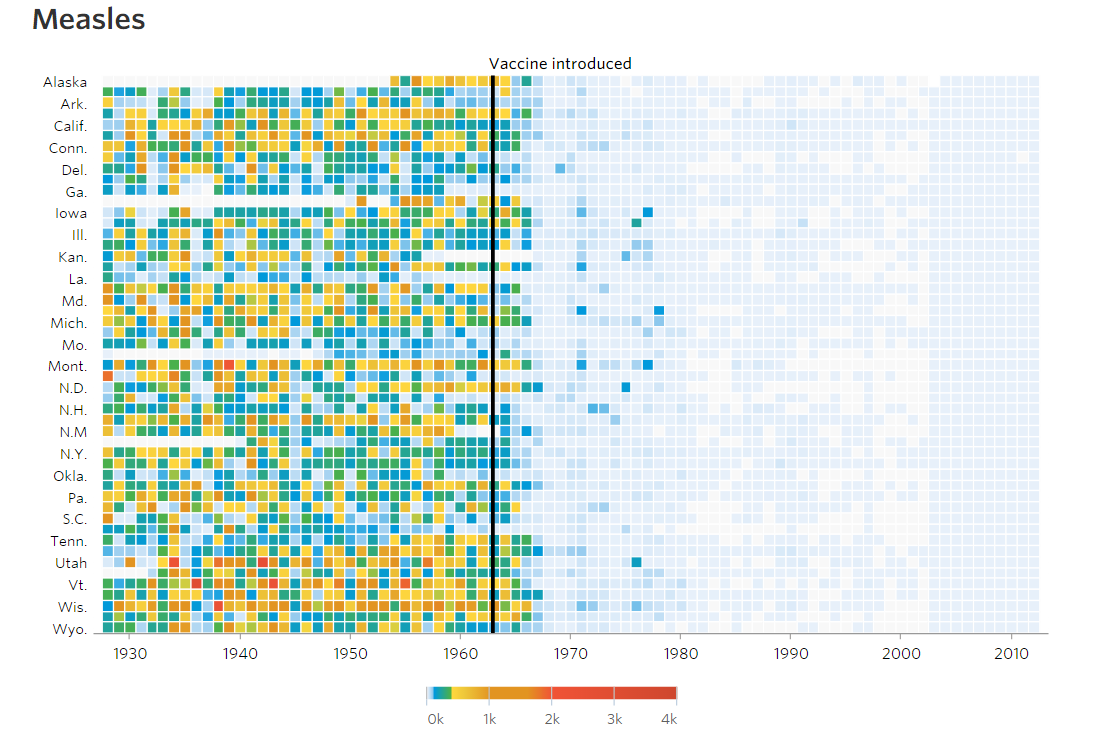
\includegraphics[width=4.5in]{\figroot/heatmap_WSJ}};
    \end{tikzpicture}
\end{frame}

\begin{frame}{What is a heatmap?}
        \textbf{Example:} Kaiser Fung's executions data

        \vspace{0.2in}

    \begin{tikzpicture}
        \node {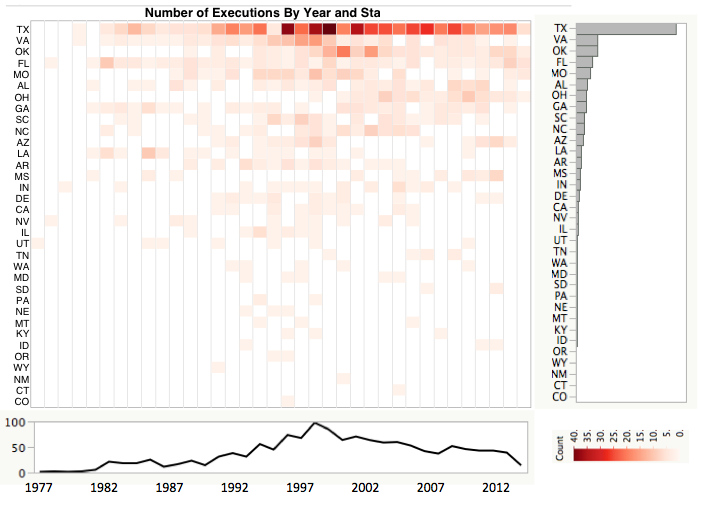
\includegraphics[width=4in]{\figroot/heatmap_KF}};
    \end{tikzpicture}
\end{frame}

\begin{frame}{What is a heatmap?}
        \textbf{Example (Bad):} A ``quilt plot'' of Hep C prevalence (Wand et al)

        \vspace{0.2in}

    \begin{tikzpicture}
        \node {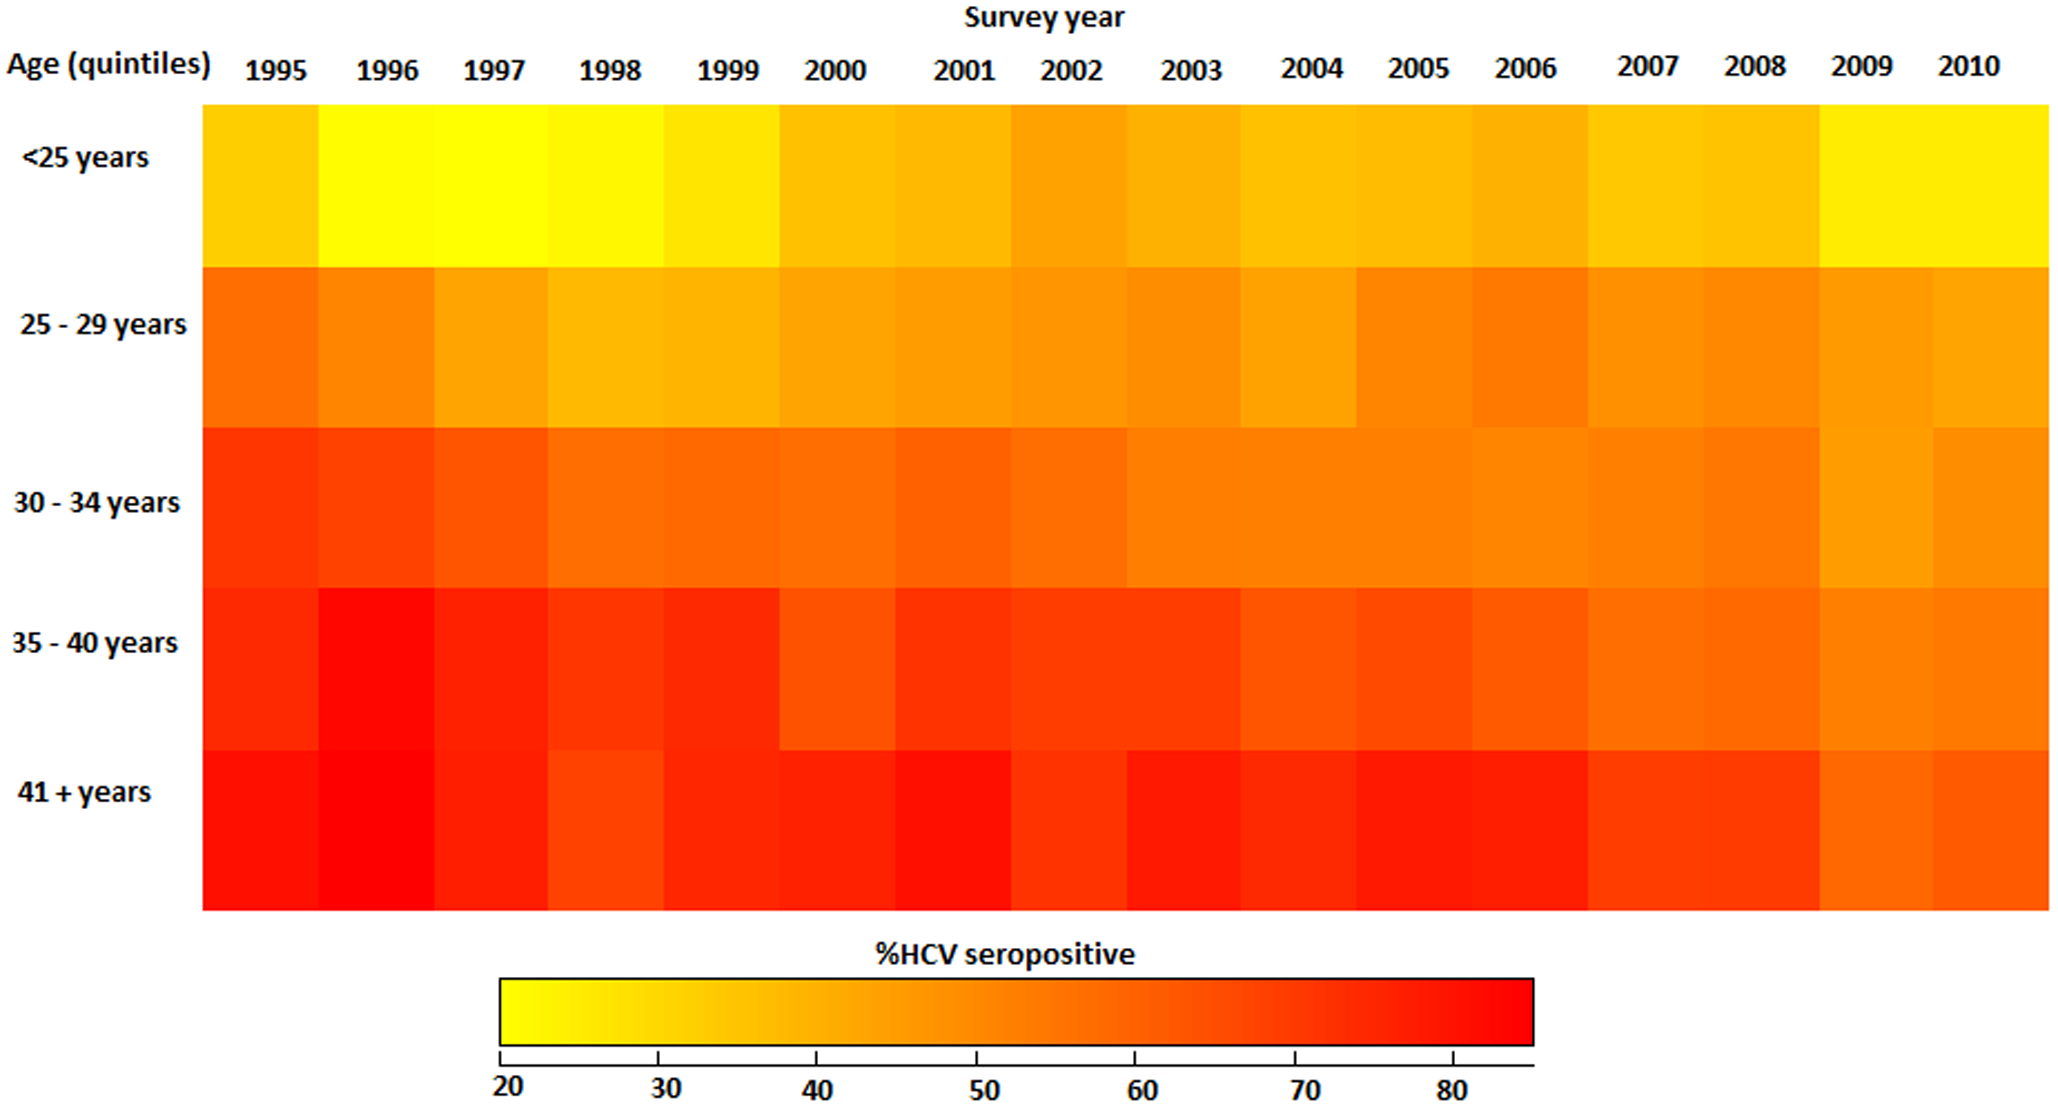
\includegraphics[width=4.2in]{\figroot/heatmap_quilt}};
    \end{tikzpicture}
\end{frame}

\begin{frame}{What is a heatmap?}

\vspace{0.2in}

    \begin{tikzpicture}[overlay]
            \node<1-> at (4.8,3.5) {\textbf{Example:} Plotting gene expression data over samples (TCGN 2013)};
        \node<1-> at (6, -0.7) {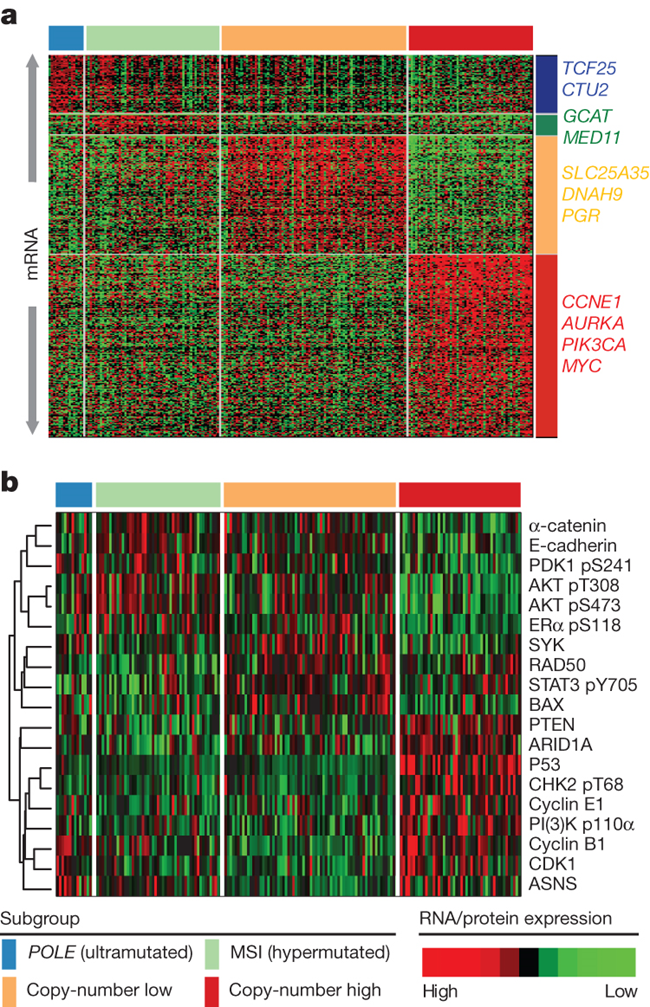
\includegraphics[height=2.8in]{\figroot/heatmap_natCGARN}};
              \onslide<2-> {\draw[thick, color=red] (3.6, -0.2) -- (3.6, 2.5);
              \node[align=left] at (1.8, 1) {Each row ($\sim$ 1500) \\ is one gene};}
        \onslide<3-> {\draw[thick, color=red] (3.6,-3.5) rectangle (4.1, -0.7);
                      \node at (1.8, -2) {\textbf{Dendrogram}};
                      \draw[thick, color=red] (8.4, -3.5) -- (8.4, -0.7);
                      \node[align=left] at (10, -2) {Each row is \\ a protein};}
    \end{tikzpicture}
\end{frame}

\begin{frame}{What is a heatmap?}
        Some takeaways from these examples:

        \begin{itemize}
                \only<1-> {\item The axes change the interpretation \newline
                      \footnotesize
                      (1) - (3) use time as the X and factors as the Y,
                      (4) uses factors for both}
               \only<2-> {\item \normalsize Good representation of high-dimensional data \newline
                       \footnotesize
                       (4) is an extreme example of this, but common in bioinformatics}
               \only<3-> {\item \normalsize Permuting axis order improves interpretation \newline
                      \footnotesize
                      (2) sorts Y by total count over the sampling period,
                      (4) uses cluster analysis (recall dendrogram)}
        \end{itemize}
\end{frame}

\begin{frame}{Setting up a heatmap for economics}

        \begin{itemize}
                \item<1-> In an ideal world, we could derive causal effects in a model $Y = g(W)$
        using exogeneous assignment of W and observing the entire support of W
                \item<2-> Big data makes the latter easier. Former still hard!
                \item<2-> Hence research designs that exploit a policy introduction or kink are popular
        \end{itemize}

        \only<3->{Now consider a heatmap where time is on the X axis (\textbf{showing the
        policy introduction}) and where W, or a variable related to a latent W,
        (\textbf{showing the support of W}) is binned on the Y axis}
\end{frame}


\begin{frame}{Setting up a heatmap for economics}
        \textbf{Example:} Scaled house sales in a heatmap sorted by FTHB exposure,
                          from Berger, Turner, Zwick ()

    \vspace{0.1in}
    \centering
    \begin{tikzpicture}
            \node {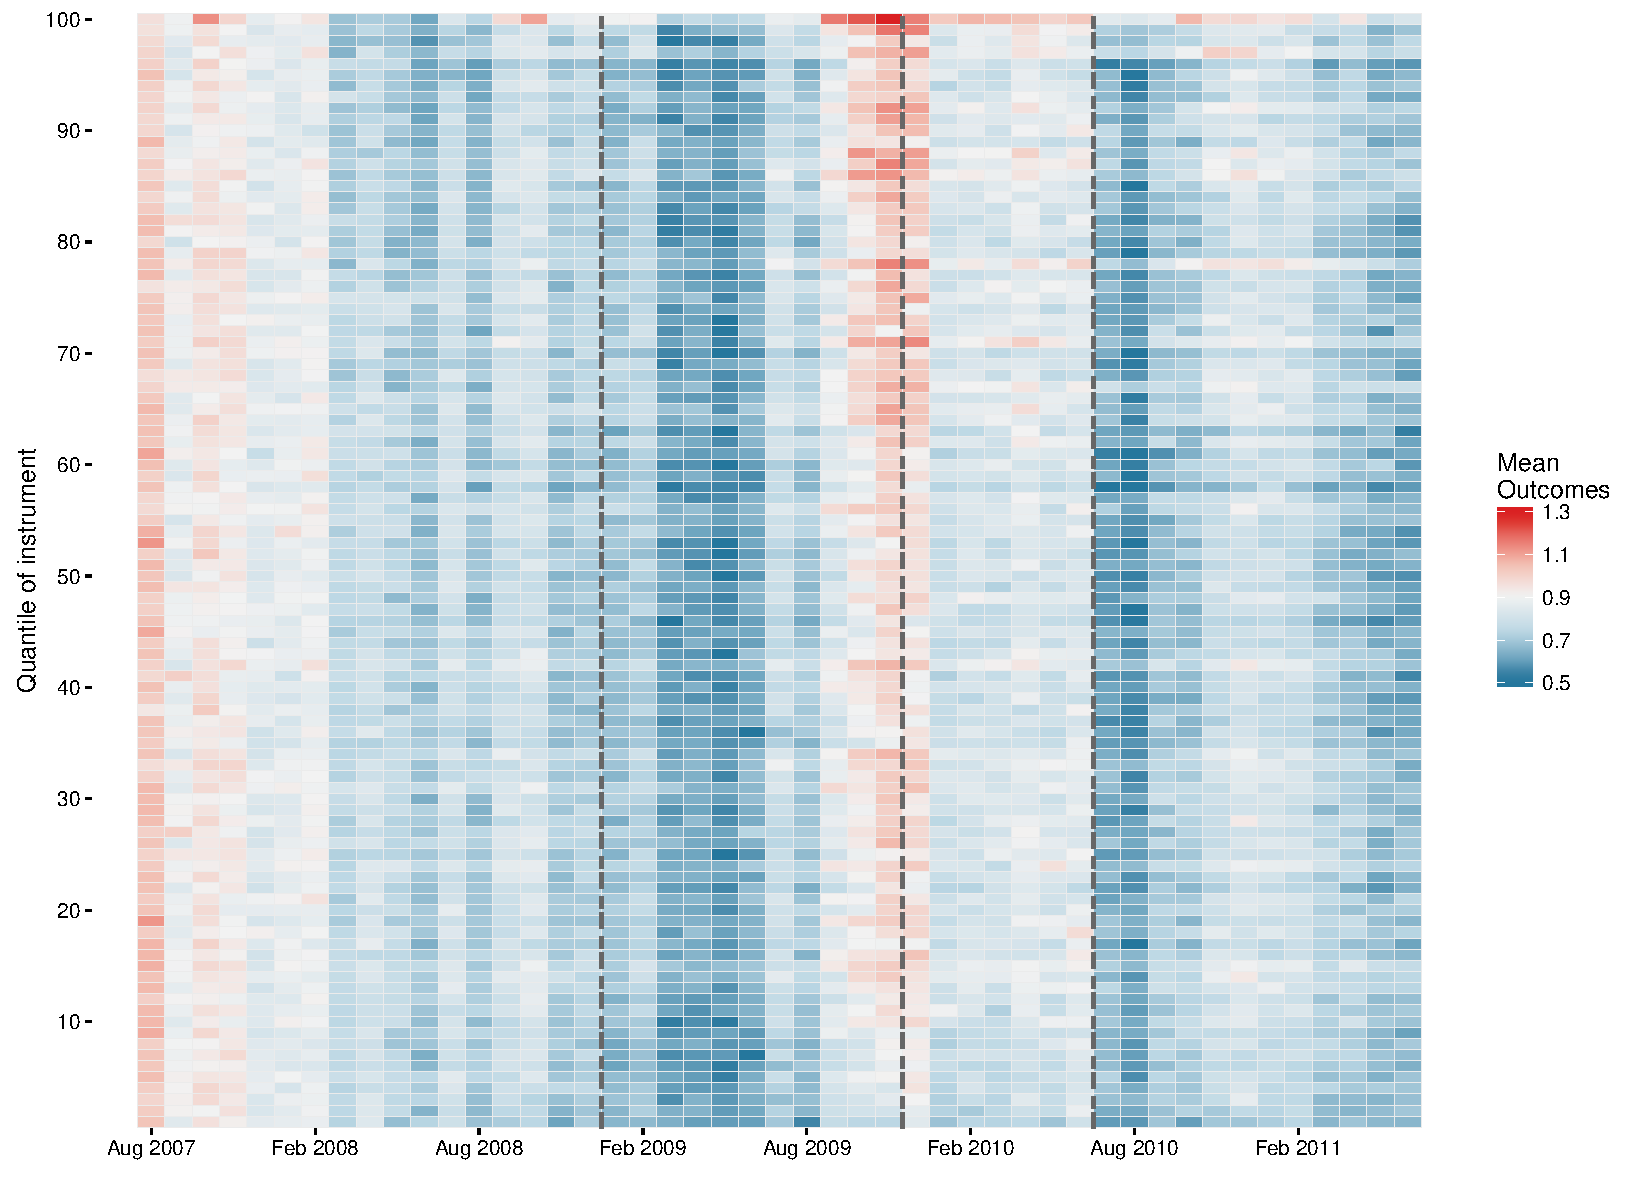
\includegraphics[width=3.8in]{\figroot/BTZRep}};
    \end{tikzpicture}

\end{frame}


\begin{frame}{Setting up a heatmap for economics}
        Using earlier takeaways:

        \begin{itemize}
                \item<1-> The axes change the interpretation \newline
                      \footnotesize
                      Placing time on X and an instrument of W on Y implies
                      this heatmap is a visualization of nonparametric regression
              \item<2-> \normalsize Good representation of high-dimensional data \newline
                       \footnotesize
                       Around ~8600 ZIPs binned into 100 percentiles
               \item<3-> \normalsize Permuting axis order improves interpretation \newline
                      \footnotesize
                      Y axis sorted to be increasing in the instrument of W,
                      and figure tells us the effect of W on Y is positive in a linear model
        \end{itemize}
\end{frame}

\begin{frame}{Setting up a heatmap for economics}
        Extensions:
        \begin{itemize}
                \item<1-> Time on X, other variables on Y, plotting means \newline = \textbf{Covariate balance check}
                \item<2-> Time on X, individual stocks on Y, plotting market-adjusted returns \newline = \textbf{Financial event study}
                \item<3-> Time on X, generation on Y, plotting average of a simulated policy function \newline = \textbf{OLG model dynamics}
                \item<4-> Policy-relevant index on X, quantiles of Y on Y, plotting obs. counts in bin \newline = \textbf{Fuzzy RDD}
        \end{itemize}
        \only<5->{and so on.}
\end{frame}

{
    \setbeamercolor{background canvas}{bg=themecolor}
\frame{
    \Large \color{white} \textbf{The heatmapEco package}
    \addtocounter{framenumber}{-1}
}
}

\begin{frame}{The heatmapEco package}
    \begin{itemize}
            \item<1-> \textbf{Many} programs for creating heatmaps exist
                    \begin{itemize}
                            \item<2-> Stata \texttt{twoway contour}, \texttt{hmap}
                            \item<2-> R base, \texttt{gplots}, \texttt{ggplot2}, \texttt{d3heatmap} \ldots
                            \item<2-> Matlab and Python \texttt{matplotlib}
                    \end{itemize}
                    So why another package?
            \onslide<3-> {\item\texttt{heatmapEco} makes informative heatmaps easy by
                    \begin{itemize}
                            \item \altcl{Focusing on proper design of axes;}
                            \item \altcl{Setting relevant axis permutations;}
                            \item \altcl{Completing prerequisite data cleaning.}
                    \end{itemize}}
    \end{itemize}
\end{frame}

\begin{frame}{The heatmapEco package}
\begin{itemize}
        \item Complicated heatmaps like TCGN's are also quite uncomplicated; they
              are literally a projection of some tabular data
        \item In other words, the data loaded in is a 373x1500 matrix. The values
              are then standardized, variables are clustered and given a colour
      \item But instead data may need to be aggregated, reshaped; axes relabelled;
       colour palettes adjusted to show significant results
       \item \texttt{heatmapEco} combines R packages to simplify these changes
              and adds design features of its own
\end{itemize}
\end{frame}

\begin{frame}{The heatmapEco package}

    \begin{tikzpicture}
            \draw[step=1, white, very thin] (0, 0) grid (10, 10);

            \fill[fill=green!12!white, rounded corners] (0.75, 6.25) rectangle (4.25, 9);
            \draw[black, thick, rounded corners] (0.75, 6.25) rectangle (4.25, 9);
            \draw (2.5, 9.2) node {Stata (heatmap)};
            \node (S2) at (2.5, 8.3) {Residualize data};
            \node (S3)[align=left] at (2.5, 7.3) {Aggregate data \\ to axis bins};
            \node (S4)[thick, align=left] at (2.5, 5.4) {OUTPUT: \\ aggregated CSV};
            \draw[->] (S2) edge (S3) (S3) edge (S4);
            \fill[fill=blue!25!white, rounded corners] (5, 2) rectangle (9, 9);
            \draw[black, thick, rounded corners] (5, 2) rectangle (9, 9);
            \draw (7, 9.2) node {R (heatmapEco)};
            \node (R2) at (7, 8.3) {Residualize data};
            \node (R3)[align=left] at (7, 7.3) {Aggregate data \\ to axis bins};
            \node (R4)[align=left] at (7, 5.4) {Aggregated table, \\ built in R or loaded};
            \node (R5) at (7, 4.3) {Axes defined w/ options};
            \node (R6)[align=left] at (7, 2.8) {heatmap built with \\ \texttt{ggplot2}};
            \node (R7)[draw, thick, text=red!85!black, align=left] at (2.5, 2.8) {OUTPUT: \\ heatmap PDF};
            \draw[->] (R2) edge (R3)  (R3) edge (R4) (R4) edge (R5)  (R5) edge (R6) (R6) edge (R7) (S4) edge (R4);
    \end{tikzpicture}

\end{frame}

\begin{frame}{heatmapEco axes}
\begin{itemize}
        \item<1-> Current support for X axis:
                \begin{itemize}
                        \item<1-> \textbf{Index axis} over numeric values (income, policy thresholds)
                        \item<1-> \textbf{Time axis} where time strings are converted into valid axis values by the package
                \end{itemize}
        \item<2-> Current support for Y axis:
                \begin{itemize}
                        \item<2-> \textbf{Factor axis} where each entry is some (aggregated) grouping
                        \item<2-> \textbf{Quantile axis} where a continuous instrument is split by N quantiles
                \end{itemize}
\end{itemize}

        \onslide<3->{Currently output is in landscape letter format, but ultimately
        axis placement should be arbitrary and portrait format heatmaps possible}
\end{frame}

\begin{frame}{heatmapEco aggregation}
\small
        \onslide<1->{In R the aggregation process is inputted using a pseudo-formula \newline
                \begin{center}
                        \texttt{Y $\sim$ CrS(X,ID,w):i(t)}
                \end{center}

        where \newline
        \begin{itemize}
                \item  \texttt{Y} is the dependent variable, or the fill variable 
                \item \texttt{X} is the factor independent variable or a continuous instrument to be binned 
                \item \texttt{i} is the index or time axis 
                \item \texttt{t} allows \texttt{X} to be sorted on its values at some time t,
                   if \texttt{X} is time varying (\textbf{use caution}) 
           \item \texttt{ID} is the individual identifier, either unique or unique with \texttt{t}
           \item \texttt{w} are quantile weights
           \end{itemize}}

        \onslide<2->{In Stata the syntax is \newline
        \texttt{heatmap Y X i [weights], id(varname) [t\_sort(string)]}}

\end{frame}

\begin{frame}{heatmapEco aggregation}
        \begin{itemize}
                \item<1-> Note that, in R, an anonymous function could be passed as an argument.
        This means the aggregation function argument \texttt{grp.func} can take
        many forms, so long as a summary function is involved
                \item<1->  E.g. take the median of a quantile-month bin. Or take the log transform
        of that median. Or add control flow; if data censored, first remove
        censored data and output log median of what remains
        \item<2->Stata's aggregation features are much less rich: every collapse
        function could be inputted into \texttt{grpfunc}
        \end{itemize}


\end{frame}


\begin{frame}{heatmapEco residualization}

        Both dependent and independent variables can be first residualized according to a model
        $$ Y = \beta W + D\theta + F\psi + X\gamma + \varepsilon $$

        Where D, F are fixed effects and X are controls.

        Stata implementation uses base \texttt{areg}. R implementation uses
        \texttt{plm} or \texttt{lfe} (TODO)
\end{frame}

\begin{frame}{Colour palettes}

    \centering
    \begin{tikzpicture}
            \node at (0, 6) {Standard divergent color palette};
            \node at (0, 4.8) {
\includegraphics[scale=0.8]{\figroot/palette.png}};
            \node at (0, 3.5) {Semi-sequential palette for count data};
            \node at (0, 2.2) {
\includegraphics[scale=0.8]{\figroot/palette_c.png}};
    \end{tikzpicture}

\footnotesize

    \begin{itemize}
            \item On standard palette, far two shades reserved for outlier detection: binned values above the 1.5 + IQR range are considerably darker
            \item Standard colors are not equally spaced: distribution below median take longer to get to dark blue hues. This is to emphasize ``Ashenfelter dips''
            \item Count data palette is ColorBrewer YlOrBr, with high outliers and
            a muted hue to deemphasize data censored by 0 (by default)
    \end{itemize}
\end{frame}

{
    \setbeamercolor{background canvas}{bg=themecolor}
\frame{
    \Large \color{white} \textbf{heatmapEco Examples}
    \addtocounter{framenumber}{-1}
}
}
\begin{frame}[fragile]{WSJ replication}
        Download data from Project Tycho. The cleaning in R:
        \small
\begin{verbatim}
library(data.table)
obj <- melt(fread("MEASLES_Incidence_1930-2003.csv"),
                  c("YEAR", "WEEK"))
obj[, value := as.numeric(value)]
\end{verbatim}

\normalsize
Calling heatmapEco:

\footnotesize

\begin{verbatim}
nasum <- function(...)
         if (all(is.na(...))) NA else sum(..., na.rm=TRUE)
heatmapEco(value ~ CrS(variable,variable):YEAR, obj,
t.fmt="\%Y", t.per="year", pol.break=c("Jan 1963"),
grp.func=nasum, count=T, factor.ax=T, outliers=T, split.x=10,
zlab="Measles Incidence (p100,000)", save="measlesRep.pdf")
\end{verbatim}

\end{frame}

\begin{frame}{WSJ replication}
\begin{tikzpicture}
    \node {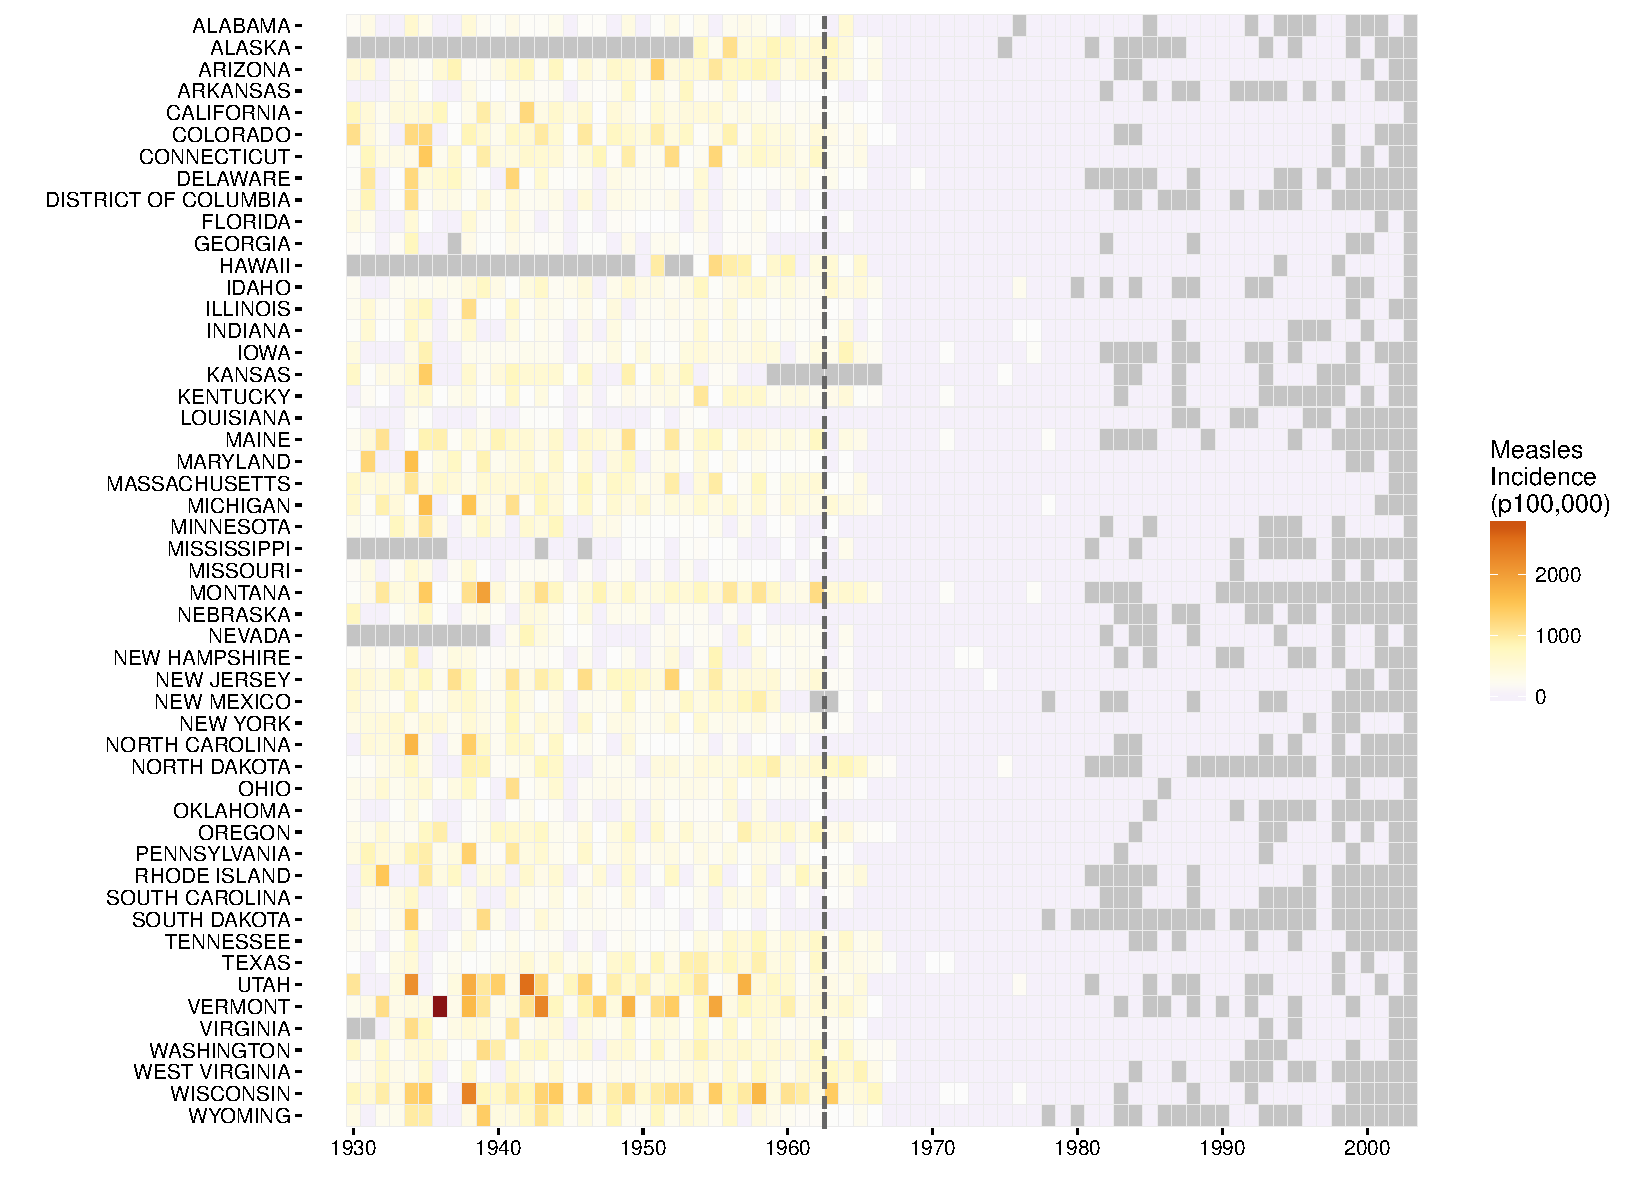
\includegraphics[width=4.5in]{\figroot/measlesRep}};
\end{tikzpicture}

\end{frame}

\begin{frame}{WSJ replication}
        \onslide<1->{Line by line:}
        \begin{itemize}
                \footnotesize
        \item<2-> \texttt{heatmapEco(value $\sim$ CrS(variable,variable):YEAR,obj, } \newline
                        Inputs formula for aggregation and dataset
        \item<2-> \texttt{t.fmt="\%Y", t.per="year", pol.break=c("Jan 1963"),} \newline
                         Data object, time is in pure ``year'' format, policy line date
                 \item<3-> \texttt{grp.func=nasum [nasum <- function(...) \newline
                  if (all(is.na(...))) NA else sum(..., na.rm=TRUE)]} \newline
                        Grouping function is summation, excluding NAs (a year with NAs is inputted as NA, grayed out)
                \item<4-> \texttt{count=T, factor.ax=T, outliers=T, split.x=10,} \newline
                      Use the count colour palette; the Y-axis are state factors; turn on outlier perception; X tick every ten units
              \item<5-> \texttt{zlab="Measles Incidence (p100,000)",save="measlesRep.pdf")} \newline
                      Policy line, labels, output location.
      \end{itemize}

      \normalsize
\onslide<7-> {Overall: \textbf{9 lines of code w/ data.table}
\begin{itemize}
        \item \textbf{9 lines fewer} than base w/ heatmap.2
        \item \textbf{~25 lines fewer} than pure ggplot2
\end{itemize}}
\end{frame}

\begin{frame}[fragile]{The Berger, Turner, Zwick heatmap}

Let's call the program from Stata this time

\footnotesize

\begin{verbatim}
heatmap y3_trim fthomebuyers_filingunits_2000 mdate ///
        [aw=totalhsales_base], n(100) id(zip) tperiod(yearmon) ///
        splity(10) polbreak(Jan 2009, Dec 2009, Jul 2010) ///
        save(BTZRep.pdf) 
\end{verbatim}

\normalsize
\begin{itemize}
        \item<1-> Default group function is mean, but the quantiles are weighted
        \item<2-> Each column is a month, labelled appropriately
        \item<3-> \texttt{polbreak()} interprets time strings and adds policy lines accordingly
        \item<4-> \texttt{splity(n)} divides y-axis labels into n even intervals
\end{itemize}


\end{frame}

\begin{frame}[fragile]{The Berger, Turner, Zwick heatmap}

\footnotesize

Another perspective: check the standard errors on the mean estimates over a coarser partition

\begin{verbatim}
heatmap y3_trim fthomebuyers_filingunits_2000 mdate ///
       [aw=totalhsales_base], n(25) id(zip) tperiod(yearmon) ///
        grpfunc(sem) splity(5) count out ///
        polbreak(Jan 2009, Dec 2009, Jul 2010) save(BTZRep_se.pdf)
\end{verbatim}

    \vspace{0.03in}
    \centering
    \begin{tikzpicture}
            \node {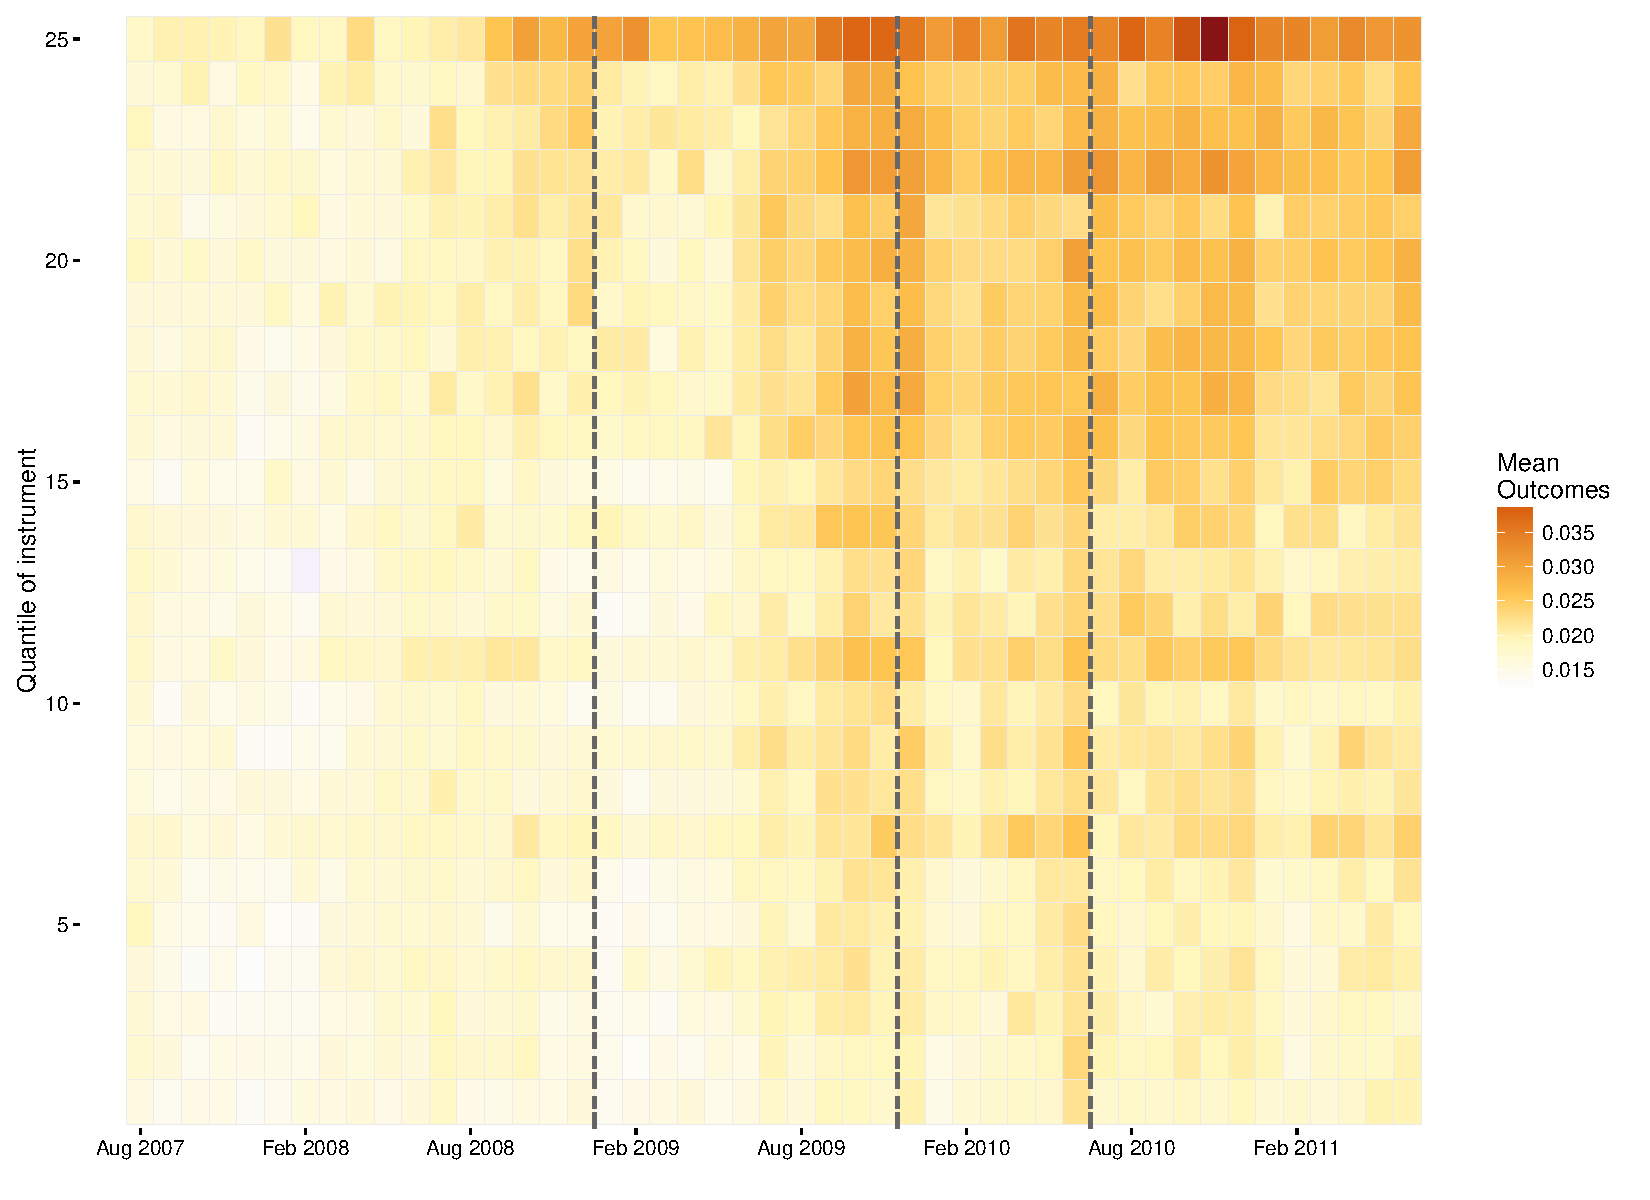
\includegraphics[width=3.1in]{\figroot/BTZRep_se}};
    \end{tikzpicture}
\end{frame}


%\begin{frame}{Event study heatmap}

        %(Want individual stocks on Y, days in X\ldots)

%\end{frame}


{
    \setbeamercolor{background canvas}{bg=themecolor}
\frame{
    \Large \color{white} \textbf{Conclusions}
    \addtocounter{framenumber}{-1}
}
}

\begin{frame}{When not to use heatmaps}

\begin{itemize}
        \item Heatmaps are not a panacea: there is a tradeoff between
                \begin{itemize}
                        \item The additional information they effectively display;
                        \item The information lost in using colours to represent change instead of geometric shapes
                \end{itemize}
        \item It is also unclear how heatmaps can display uncertainty of estimates:
              distribution of estimates, e.g.?
        \item A good argument for a package that simplifies heatmap creation ---
              the less time spent making a visualization, the less likely
              one gets overattached to one when a better solution exists
\end{itemize}
\end{frame}

\begin{frame}{When not to use heatmaps}

A good heuristic (define Z as the variable plotted with colour):
                \begin{itemize}
                      \item Plotting quantiles on the Y axis:
                            Is your graph confounded if you plotted Z against X
                            in overlapping line graphs split by Y?
                        \item Plotting a factor variable on the Y axis:
                              Is your graph confounded if you plotted Z against X
                              in a small multiples plot split by Y?
                \end{itemize}
\end{frame}

\begin{frame}{When not to use heatmaps}

\textbf{Example}: Measles vaccine revisited

\begin{tikzpicture}
\node {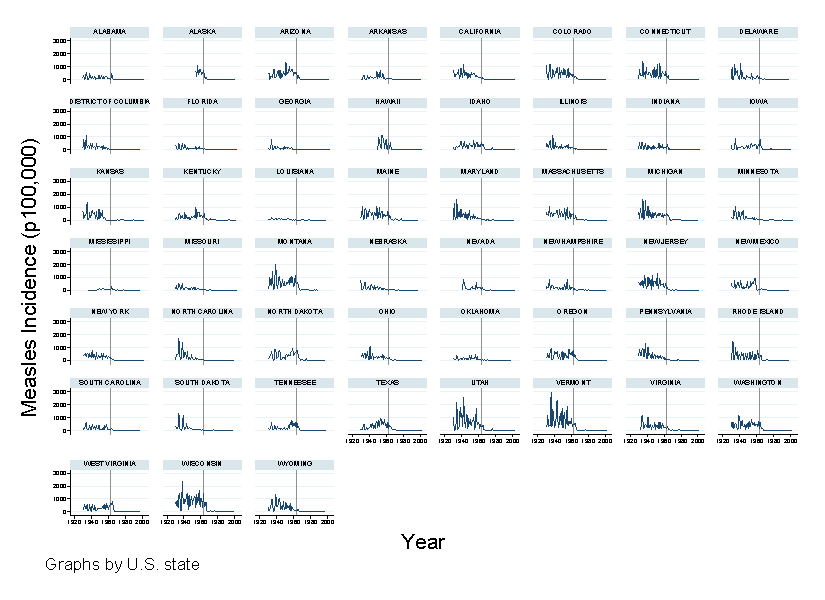
\includegraphics[width=4in]{\figroot/measlesSM}};
\end{tikzpicture}

\end{frame}


\begin{frame}{When not to use heatmaps}

\textbf{Example}: visualizing positive assortative matching

\begin{tikzpicture}
\node {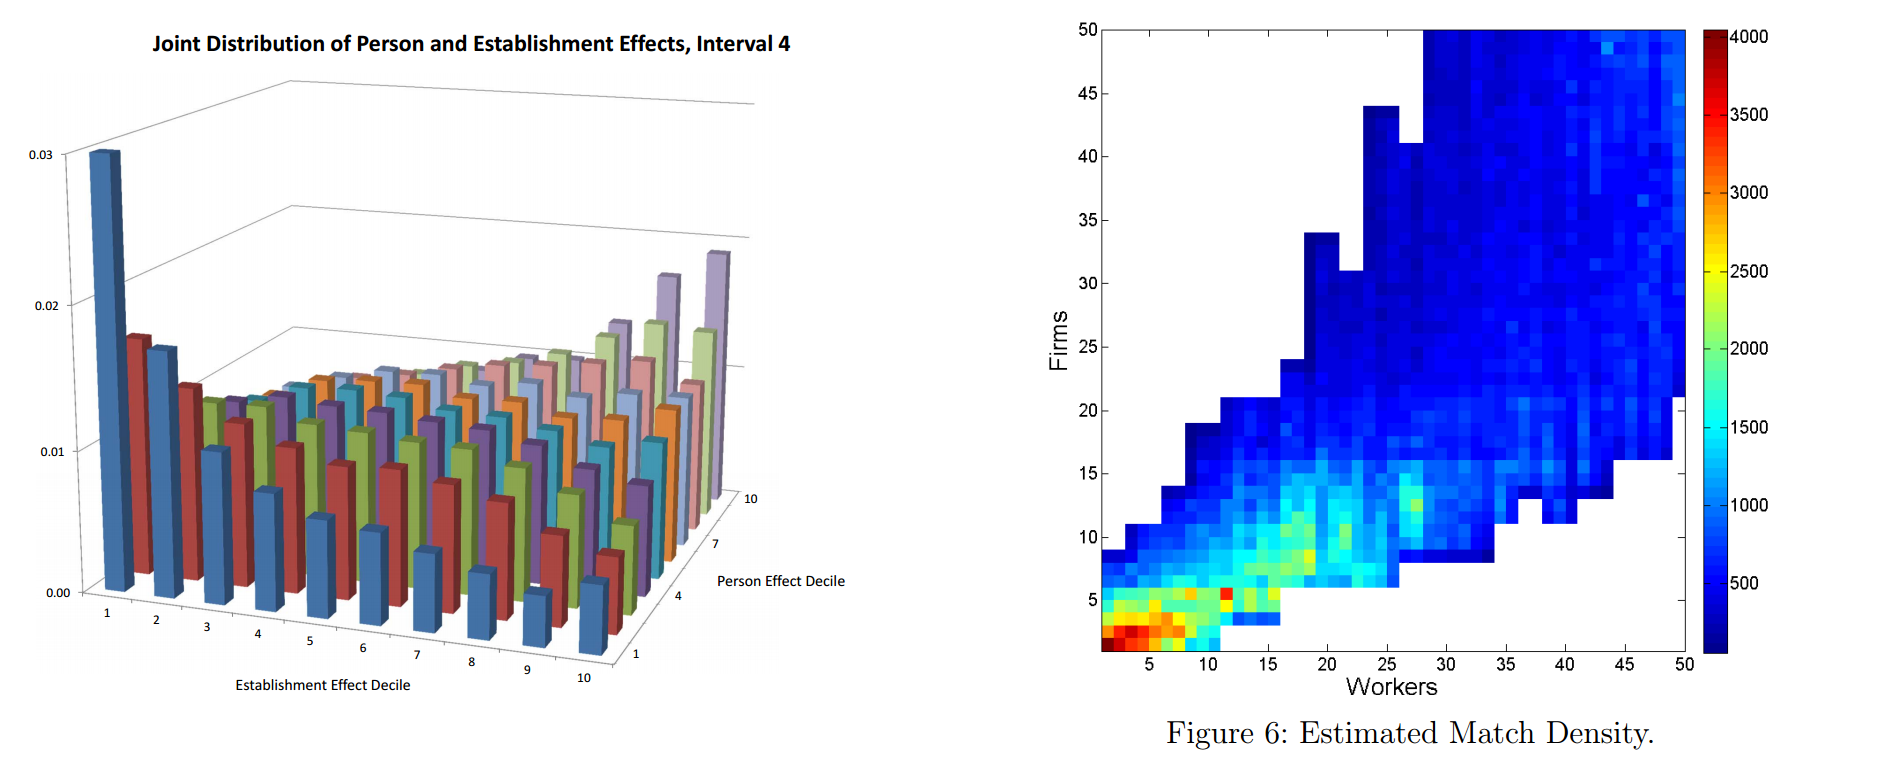
\includegraphics[width=4.5in]{\figroot/matching_CardVsHLM}};
\end{tikzpicture}

\footnotesize

(L: Card, Heining \& Kline (2012); R: Hagedorn, Law \& Manovskii (2016))

\normalsize
2016
How would the interpretation change if the visualization was instead
overlaying many marginals over each other? Small multiples of marginals?

\end{frame}





\begin{frame}{Future updates}

\begin{itemize}
        \item Syntax revisions
        \item Complementary side plots (histograms, time series, diffs\ldots)
        \item Both axes can belong in one of four types
        \item Port the heatmap palette for utilisation in base R heatmap f'n
        \item ???
\end{itemize}

\end{frame}

\begin{frame}{References}

\end{frame}

%< Thanks
{
    \setbeamercolor{background canvas}{bg=themecolor}
\frame{
    \Huge \color{white} Thanks!
    \addtocounter{framenumber}{-1}
}
}

\end{document}

